\documentclass[11pt]{article}
\usepackage[table]{xcolor}
\usepackage{amsmath} 
\usepackage{graphicx}
\usepackage{subcaption}
\usepackage{sectsty}
\usepackage{amssymb}
 \usepackage{lipsum}
\usepackage{titlesec}
\usepackage{romannum}
\usepackage{enumitem}
\usepackage{mathtools}
\usepackage[super]{nth}
\usepackage{tikz}
\usepackage{listings}
\usepackage{pagecolor,lipsum}
\usepackage{color,soul}
\usepackage{xcolor}
\usepackage{hyperref}
\usepackage[T1]{fontenc}
\usepackage{textcomp}
\usepackage{float}
\usepackage{media9}
\usepackage[utf8]{inputenc}
\usepackage[T1]{fontenc}
\usepackage{parskip}

\definecolor{theWhite}{gray}{0.9}
\definecolor{theBlack}{gray}{0.0}
\definecolor{dkgreen}{rgb}{0,0.6,0}
\definecolor{gray}{rgb}{0.5,0.5,0.5}
\definecolor{mauve}{rgb}{0.58,0,0.82}
\definecolor{codegreen}{rgb}{0,0.6,0}
\definecolor{codegray}{rgb}{0.5,0.5,0.5}
\definecolor{codepurple}{rgb}{0.58,0,0.82}
\definecolor{backcolour}{rgb}{0.95,0.95,0.92}
\definecolor{orange}{RGB}{255,127,0}
%\definecolor{lightgray}{rgb}{0.95, 0.95, 0.95}
\definecolor{darkgray}{rgb}{0.4, 0.4, 0.4}
%\definecolor{purple}{rgb}{0.65, 0.12, 0.82}
\definecolor{editorGray}{rgb}{0.95, 0.95, 0.95}
\definecolor{editorOcher}{rgb}{1, 0.5, 0} % #FF7F00 -> rgb(239, 169, 0)
\definecolor{editorGreen}{rgb}{0, 0.5, 0} % #007C00 -> rgb(0, 124, 0)
\definecolor{orange}{rgb}{1,0.45,0.13}		
\definecolor{olive}{rgb}{0.17,0.59,0.20}
\definecolor{brown}{rgb}{0.69,0.31,0.31}
\definecolor{purple}{rgb}{0.38,0.18,0.81}
\definecolor{lightblue}{rgb}{0.1,0.57,0.7}
\definecolor{lightred}{rgb}{1,0.4,0.5}
\pagecolor{white}
\graphicspath{ {./images/} }
\setlength{\fboxsep}{1pt}

\lstdefinelanguage{Comment}{
  identifierstyle=\color{white},
  sensitive=false,
}

% CSS
\lstdefinelanguage{CSS}{
  keywords={color,background-image:,margin,padding,font,weight,display,position,top,left,right,bottom,list,style,border,size,white,space,min,width, transition:, transform:, transition-property, transition-duration, transition-timing-function},	
  sensitive=true,
  morecomment=[l]{//},
  morecomment=[s]{/*}{*/},
  morestring=[b]',
  morestring=[b]",
  alsoletter={:},
  alsodigit={-}
}

% JavaScript
\iffalse
\lstdefinelanguage{JavaScript}{
  morekeywords={typeof, new, true, false, catch, function, return, null, catch, switch, var, if, while, do, else, case, break},
  morecomment=[s]{/*}{*/},
  morecomment=[l]//,
  morestring=[b]",
  morestring=[b]'
}
\fi

\lstdefinelanguage{HTML5}{
  language=html,
  sensitive=true,	
  alsoletter={<>=-},	
  morecomment=[s]{<!-}{-->},
  tag=[s],
  otherkeywords={
  % General
  >,
  % Standard tags
	<!DOCTYPE,
  </html, <html, <head, <title, </title, <style, </style, <link, </head, <meta, />,
	% body
	</body, <body,
	% Divs
	</div, <div, </div>, 
	% Paragraphs
	</p, <p, </p>,
	% scripts
	</script, <script,
	% 
	<h1, </h1,
	<span, </span,
	<strong, </strong,
	<em, </em, 
	<br, 
	<ul, </ul, 
	<li, </li, 
	<ol, </ol, 
	<img, 
	</video, 
	html>, 
	<a, </a, 
	<table, </table,
	<tr, </tr, 
	<td, </td, 
	<th, </th, 
	<tbody, </tbody, 
	<thead, </thead, 
	<tfoot, </tfoot, 
	<form, </form,
	<input, </input,
	<label, </label, 
	<select, </select, 
	<option, </option, 
	<textarea, </textarea, 
  % More tags...
  <canvas, /canvas>, <svg, <rect, <animateTransform, </rect>, </svg>, <video, <source, <iframe, </iframe>, </video>, <image, </image>, <header, </header, <article, </article
  },
  ndkeywords={
  % General
  =,
  % HTML attributes
  charset=, src=, id=, width=, height=, style=, type=, rel=, href=, alt=, controls, target=, border=, colspan=, rowspan=, scope=, action=, method=, name=, value=, for=, step=, min=, max=, rows=, 
  cols=, 
  % SVG attributes
  fill=, attributeName=, begin=, dur=, from=, to=, poster=, controls=, x=, y=, repeatCount=, xlink:href=,
  % properties
  margin:, padding:, background-image:, border:, top:, left:, position:, width:, height:, margin-top:, margin-bottom:, font-size:, line-height:, font-family:, text-align:, 
	% CSS3 properties
  transform:, -moz-transform:, -webkit-transform:,
  animation:, -webkit-animation:,
  transition:,  transition-duration:, transition-property:, transition-timing-function:,
  }
}

\lstset {%
  % General design
  backgroundcolor=\color{backcolour},
  basicstyle={\small\ttfamily},   
  %frame=b,
  % line-numbers
  xleftmargin={0.75cm},
  numbers=left,
  stepnumber=1,
  firstnumber=1,
  numberfirstline=true,	
  % Code design
  identifierstyle=\color{black},
  keywordstyle=\color{blue}\bfseries,
  ndkeywordstyle=\color{editorGreen}\bfseries,
  stringstyle=\color{editorOcher}\ttfamily,
  commentstyle=\color{brown}\ttfamily,
  % Code
  language=HTML5,
  %alsolanguage=JavaScript,
  alsodigit={.:;},	
  tabsize=2,
  showtabs=false,
  showspaces=false,
  showstringspaces=false,
  extendedchars=true,
  breaklines=true,
  % German umlauts
  literate=%
  {Ö}{{\"O}}1
  {Ä}{{\"A}}1
  {Ü}{{\"U}}1
  {ß}{{\ss}}1
  {ü}{{\"u}}1
  {ä}{{\"a}}1
  {ö}{{\"o}}1
}

\newcommand*\circled[1]{\tikz[baseline=(char.base)]{
            \node[shape=circle,draw,inner sep=2pt] (char) {#1};}}
\setlength\parindent{0pt}
\setlist[itemize,1]{leftmargin=\dimexpr 26pt-.5in}

\sectionfont{\fontsize{12}{15}\selectfont}
\title{Introduction to Programming with Javascript}
\author{Qitian Liao}
\date{Aug 3, 2020} 
\usepackage[left=2cm, right=2cm, top=2cm]{geometry}
%\setlength\parindent{0pt}

\DeclarePairedDelimiter\abs{\lvert}{\rvert}
\DeclarePairedDelimiter\norm{\lVert}{\rVert}

\begin{document}
\begin{titlepage}
	\begin{center} 
	\line(1, 0){400}\\
	[0.25in]
	\huge{\bfseries Introduction to HTML} \\
	[2mm]
	\line(1, 0){300} \\
	[1.5cm]
	\textsc{\LARGE Qitian Liao} \\
	[0.5cm]
	\textsc{\large University of California, Berkeley} \\
	[15cm]
	\end{center}
	\begin{flushright}	
	\end{flushright}
\end{titlepage}

\thispagestyle{empty}
\newpage
\tableofcontents
\thispagestyle{empty}
\cleardoublepage
\setcounter{page}{1}
\def\Arg{\mathop{\operator@font Arg}\nolimits}
\pagenumbering{arabic}
\titleformat*{\section}{\Large\bfseries}
\titleformat*{\subsection}{\large\bfseries}
\titleformat*{\subsubsection}{\normalsize\bfseries}
\titleformat*{\paragraph}{\large\bfseries}
\titleformat*{\subparagraph}{\large\bfseries}
\newpage

\section{Introduction to HTML}
Now we will learn the basic structure of an HTML document.
\subsection{Introduction to HTML}
HTML is the skeleton of all web pages. It is often the first language learned by developers, marketers, and designers and is core to front-end development work. HTML provides structure to the content appearing on a website, such as images, text, or videos. Right-click on any page on the internet, choose “Inspect,” and we will see HTML in a panel of your screen. 

HTML stands for HyperText Markup Language:
\begin{itemize}[leftmargin = *]
\item A \textit{markup} language is a computer language that defines the structure and presentation of raw text.
\item In HTML, the computer can interpret \textit{raw text} that is wrapped in HTML elements.
\item \textit{HyperText} is text displayed on a computer or device that provides access to other text through links, also known as \textit{hyperlinks}. 
\end{itemize}
Learning HTML is the first step in creating websites, but even a bit of knowledge can help us inject code snippets into newsletter, blog or website templates. As we continue learning, we can layer HTML with CSS and JavaScript to create visually compelling and dynamic websites. Now, we are going to focus on how to add and modify basic content on a page, like text, images, and videos.

\subsection{HTML Anatomy}
HTML is composed of \textit{elements}. These elements structure the webpage and define its content. Let us take a look at how they are written.
\begin{figure}[H]
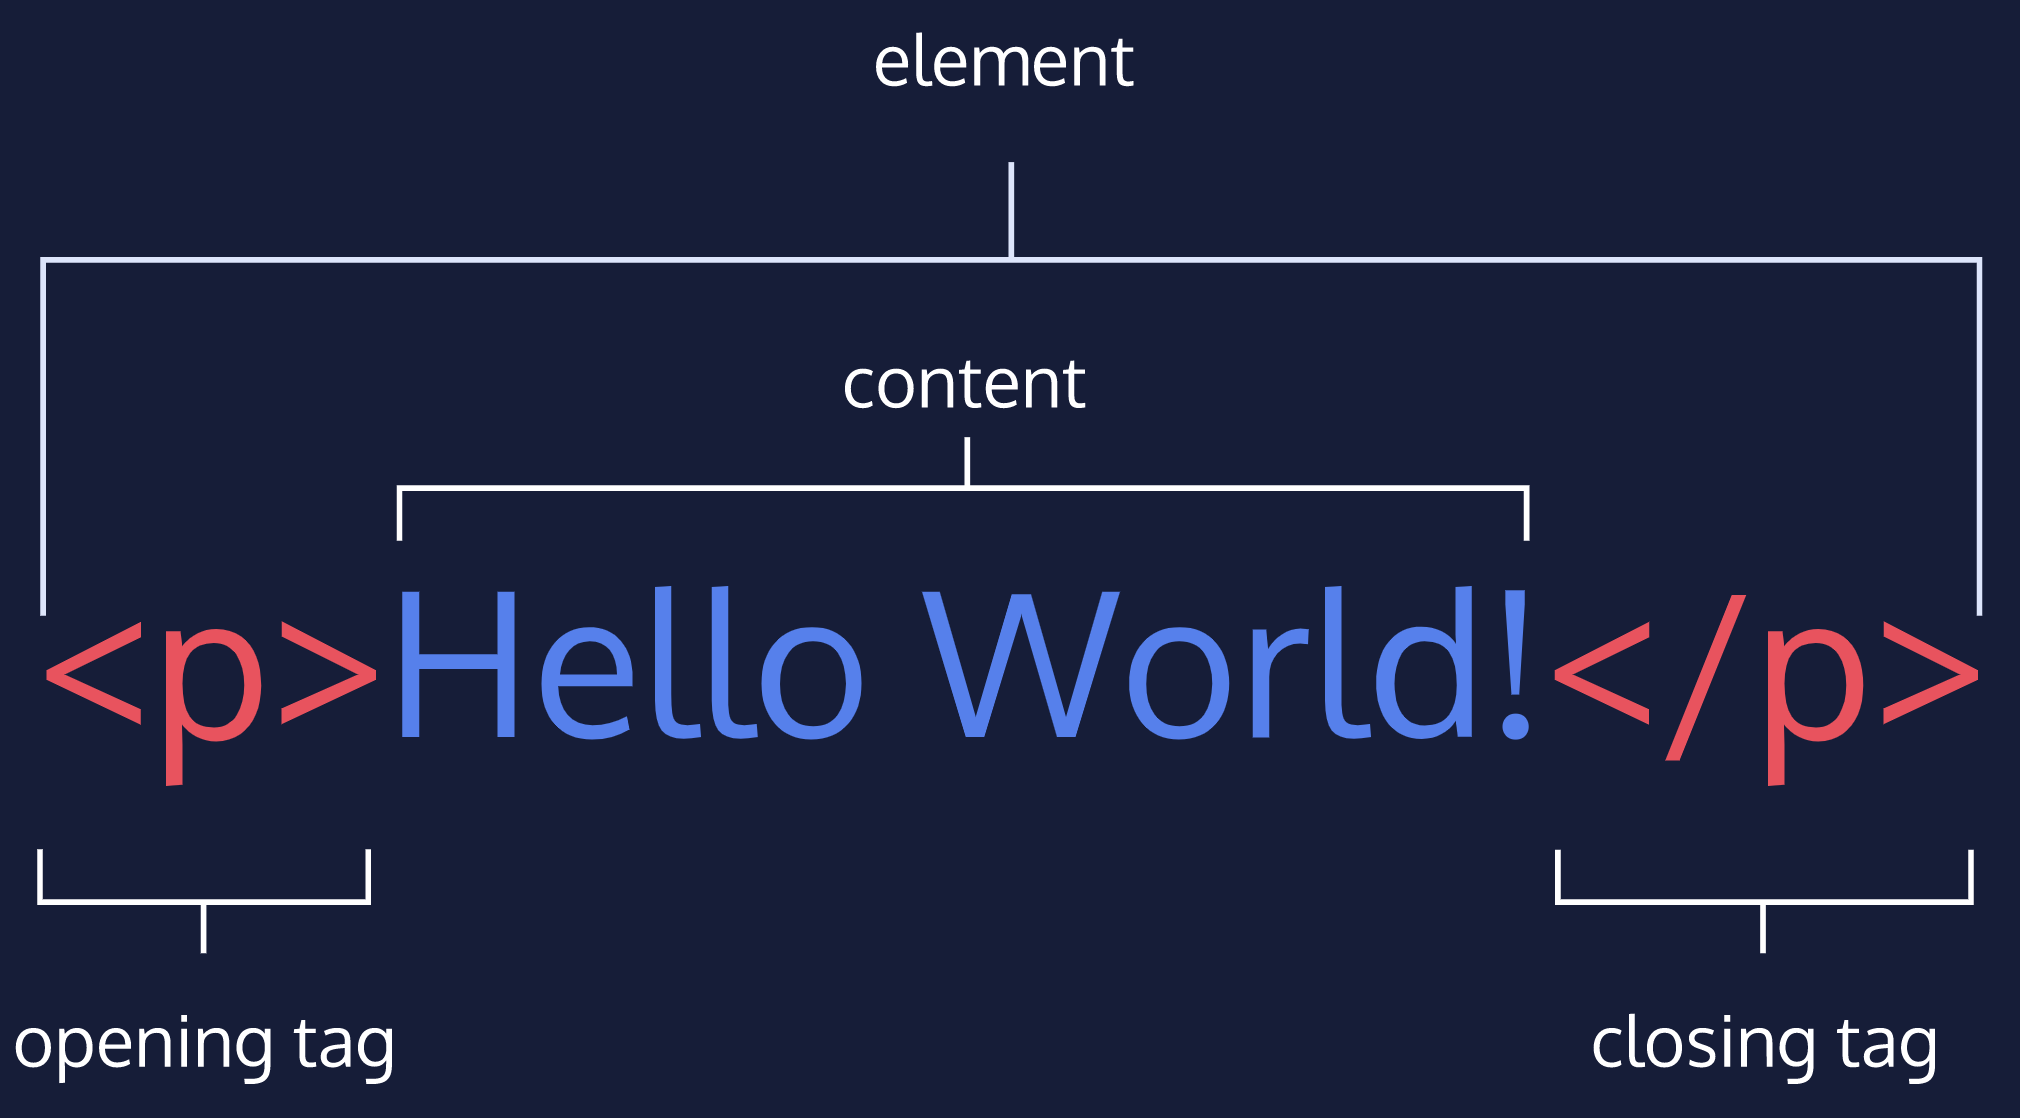
\includegraphics[scale = 0.2]{1_1}
\centering
\end{figure}
The diagram above displays an HTML paragraph element. As we can see, the paragraph element is made up of:
\begin{itemize}[leftmargin = *]
\item An \textit{opening tag} (\colorbox{lightgray}{<p>})
\item The content (“Hello World!” text)
\item A \textit{closing tag} (\colorbox{lightgray}{<$/$p>})
\end{itemize}
A \textit{tag} and the \textit{content} between it is called an HTML element. There are many tags that we can use to organize and display text and other types of content, like images. 

Let us quickly review each part of the element pictured:
\begin{itemize}[leftmargin = *]
\item HTML element (or simply, element) — a unit of content in an HTML document formed by HTML tags and the text or media it contains.
\item HTML Tag — the element name, surrounded by an opening (\colorbox{lightgray}{<}) and closing (\colorbox{lightgray}{>}) angle bracket. 
\item Opening Tag — the first HTML tag used to start an HTML element. The tag type is surrounded by opening and closing angle brackets.
\item Content — The information (text or other elements) contained between the opening and closing tags of an HTML element.
\item Closing tag — the second HTML tag used to end an HTML element. Closing tags have a forward slash (\colorbox{lightgray}{$/$}) inside of them, directly after the left angle bracket.
\end{itemize}

\subsection{The Body}
One of the key HTML elements we use to build a webpage is the \textit{body} element. Only content inside the opening and closing body tags can be displayed to the screen. Here is what opening and closing body tags look like:
\begin{lstlisting}
<body>

</body>
\end{lstlisting}
Once the file has a body, many different types of content – including text, images, and buttons – can be added to the body.
\begin{lstlisting}
<body>
  <p>Hello, doc!</p>
</body>
\end{lstlisting}

\subsection{HTML Structure}
HTML is organized as a collection of family tree relationships. As you saw in the last exercise, we placed \colorbox{lightgray}{<p>} tags within \colorbox{lightgray}{<body>} tags. When an element is contained inside another element, it is considered the \textit{child} of that element. The child element is said to be \textit{nested} inside of the \textit{parent} element.
\begin{lstlisting}
<body>
  <p>This paragraph is a child of the body</p>
</body>
\end{lstlisting}
In the example above, the \colorbox{lightgray}{<p>} element is nested inside the \colorbox{lightgray}{<body>} element. The \colorbox{lightgray}{<p>} element is considered a child of the \colorbox{lightgray}{<body>} element, and the \colorbox{lightgray}{<body>} element is considered the parent. Notice that we have added two spaces of indentation (using the \framebox[1.1\width]{space} bar) for better readability. 

Since there can be multiple levels of nesting, this analogy can be extended to grandchildren, great-grandchildren, and beyond. The relationship between elements and their ancestor and descendent elements is known as \textit{hierarchy}. 

Let us consider a more complicated example that uses some new tags: 
\begin{lstlisting}
<body>
  <div>
    <h1>Sibling to p, but also grandchild of body</h1>
    <p>Sibling to h1, but also grandchild of body</p>
  </div>
</body>
\end{lstlisting}
In this example, the \colorbox{lightgray}{<body>} element is the parent of the \colorbox{lightgray}{<div>} element. Both the \colorbox{lightgray}{<h1>} and \colorbox{lightgray}{<p>} elements are children of the \colorbox{lightgray}{<div>} element. Because the \colorbox{lightgray}{<h1>} and \colorbox{lightgray}{<p>} elements are at the same level, they are considered siblings and are both grandchildren of the \colorbox{lightgray}{<body>} element.

Understanding HTML hierarchy is important because child elements can inherit behavior and styling from their parent element. We will learn more about webpage hierarchy when you start digging into CSS.

\subsection{Headings}
Headings in HTML are similar to headings in other types of media. For example, in newspapers, large headings are typically used to capture a reader’s attention. Other times, headings are used to describe content, like the title of a movie or an educational article.

HTML follows a similar pattern. In HTML, there are six different \textit{headings}, or \textit{heading elements}. Headings can be used for a variety of purposes, like titling sections, articles, or other forms of content.

The following is the list of heading elements available in HTML. They are ordered from largest to smallest in size.
\begin{enumerate}[leftmargin = *]
\item \colorbox{lightgray}{<h1>} — used for main headings. All other smaller headings are used for subheadings.
\item \colorbox{lightgray}{<h2>}
\item \colorbox{lightgray}{<h3>}
\item \colorbox{lightgray}{<h4>}
\item \colorbox{lightgray}{<h5>}
\item \colorbox{lightgray}{<h6>}
\end{enumerate}
The following example code uses a headline intended to capture a reader’s attention. It uses the largest heading available, the main heading element:
\begin{lstlisting}
<h1>BREAKING NEWS</h1>
\end{lstlisting}

\subsection{Divs}
One of the most popular elements in HTML is the \colorbox{lightgray}{<div>} element. \colorbox{lightgray}{<div>} is short for “division” or a container that divides the page into sections. These sections are very useful for grouping elements in your HTML together.
\begin{lstlisting}
<body>
  <div>
    <h1>Why use divs?</h1>
    <p>Great for grouping elements!</p>
  </div>
</body>
\end{lstlisting}
\colorbox{lightgray}{<div>}s can contain any text or other HTML elements, such as links, images, or videos. Remember to always add two spaces of indentation when you nest elements inside of \colorbox{lightgray}{<div>}s for better readability.

\subsection{Attributes}
If we want to expand an element’s tag, we can do so using an \textit{attribute}. Attributes are content added to the opening tag of an element and can be used in several different ways, from providing information to changing styling. Attributes are made up of the following two parts:
\begin{itemize}[leftmargin = *]
\item The \textit{name} of the attribute
\item The \textit{value} of the attribute
\end{itemize}
One commonly used attribute is the \colorbox{lightgray}{id}. We can use the \colorbox{lightgray}{id} attribute to specify different content (such as \colorbox{lightgray}{<div>}s) and is really helpful when you use an element more than once. \colorbox{lightgray}{id}s have several different purposes in HTML, but for now, we will focus on how they can help us identify content on our page.

When we add an \colorbox{lightgray}{id} to a \colorbox{lightgray}{<div>}, we place it in the opening tag:
\begin{lstlisting}
<div id="intro">
  <h1>Introduction</h1>
</div>
\end{lstlisting}

\subsection{Displaying Text}
If you want to display text in HTML, you can use a \textit{paragraph} or \textit{span}:
\begin{itemize}[leftmargin = *]
\item \textit{Paragraphs} (\colorbox{lightgray}{<p>}) contain a block of plain text.
\item \colorbox{lightgray}{<span>} contains short pieces of text or other HTML. They are used to separate small pieces of content that are on the same line as other content.
\end{itemize}
Take a look at each of these elements in action below:
\begin{lstlisting}
<div>
  <h1>Technology</h1>
</div>
<div>
  <p><span>Self-driving cars</span> are anticipated to 
  replace up to 2 million jobs over the next two decades.</p>
</div>
\end{lstlisting}
In the example above, there are two different \colorbox{lightgray}{<div>}. The second \colorbox{lightgray}{<div>} contains a \colorbox{lightgray}{<p>} with \\
\colorbox{lightgray}{<span>Self-driving cars</span>}. This \colorbox{lightgray}{<span>} element separates “Self-driving cars” from the rest of the text in the paragraph.

It is best to use a \colorbox{lightgray}{<span>} element when you want to target a specific piece of content that is inline, or on the same line as other text. If you want to divide your content into blocks, it is better to use a \colorbox{lightgray}{<div>}.

\subsection{Styling Text}
You can also style text using HTML tags. The \colorbox{lightgray}{<em>} tag emphasizes text, while the \colorbox{lightgray}{<strong>} tag highlights important text.

Later, when we begin to style websites, we will decide how you want browsers to display content within \colorbox{lightgray}{<em>} and \colorbox{lightgray}{<strong>} tags. Browsers, however, have built-in style sheets that will generally style these tags in the following ways:
\begin{itemize}[leftmargin = *]
\item The \colorbox{lightgray}{<em>} tag will generally render as italic emphasis.
\item The \colorbox{lightgray}{<strong>} will generally render as bold emphasis.
\end{itemize}
Take a look at each style in action:
\begin{lstlisting}
<p><strong>The Nile River</strong> is the <em>longest</em> 
river in the world, measuring over 6,850 kilometers long 
(approximately 4,260 miles).</p>
\end{lstlisting}
In this example, the \colorbox{lightgray}{<strong>} and \colorbox{lightgray}{<em>} tags are used to emphasize the text to produce the following:
\vspace{-3mm}
\par\noindent\rule{\textwidth}{0.2pt}
\textbf{The Nile River} is the \textit{longest} river in the world, measuring over 6,850 kilometers long (approximately 4,260 miles).
\vspace{-3mm}
\par\noindent\rule{\textwidth}{0.2pt}
As we can see, “The Nile River” is bolded and “longest” is in italics.

\subsection{Line Breaks}
The spacing between code in an HTML file does not affect the positioning of elements in the browser. If you are interested in modifying the spacing in the browser, you can use HTML’s \textit{line break} element: \colorbox{lightgray}{<br>}.

The line break element is unique because it is only composed of a starting tag. You can use it anywhere within your HTML code and a line break will be shown in the browser.
\begin{lstlisting}
<p>The Nile River is the longest river <br> in the world, 
measuring over 6,850 <br> kilometers long (approximately 
4,260 <br> miles).</p>
\end{lstlisting}
The code in the example above will result in an output that looks like the following:
\vspace{-3mm}
\par\noindent\rule{\textwidth}{0.2pt}
The Nile River is the longest river \\ 
in the world, measuring over 6,850 \\ 
kilometers long (approximately 4,260 \\
miles).
\vspace{-3mm}
\par\noindent\rule{\textwidth}{0.2pt}

\subsection{Unordered Lists}
In addition to organizing text in paragraph form, you can also display content in an easy-to-read list.

In HTML, you can use an \textit{unordered list} tag (\colorbox{lightgray}{<ul>}) to create a list of items in no particular order. An unordered list outlines individual list items with a bullet point.

The \colorbox{lightgray}{<ul>} element should not hold raw text and will not automatically format raw text into an unordered list of items. Individual list items must be added to the unordered list using the \colorbox{lightgray}{<li>} tag. The \colorbox{lightgray}{<li>} or list item tag is used to describe an item in a list.
\begin{lstlisting}
<ul>
  <li>Limes</li>
  <li>Tortillas</li>
  <li>Chicken</li>
</ul>
\end{lstlisting}
In the example above, the list was created using the \colorbox{lightgray}{<ul>} tag and all individual list items were added using \colorbox{lightgray}{<li>} tags.

The output will look like this:
\vspace{-3mm}
\par\noindent\rule{\textwidth}{0.2pt}
\begin{itemize}[leftmargin = 24pt]
\item Limes
\item Tortillas
\item Chicken
\end{itemize}
\vspace{-3mm}
\par\noindent\rule{\textwidth}{0.2pt}

\subsection{Ordered Lists}
\textit{Ordered lists} (\colorbox{lightgray}{<ol>}) are like unordered lists, except that each list item is numbered. They are useful when you need to list different steps in a process or rank items for first to last.

You can create the ordered list with the \colorbox{lightgray}{<ol>} tag and then add individual list items to the list using \colorbox{lightgray}{<li>} tags.
\begin{lstlisting}
<ol>
  <li>Preheat the oven to 350 degrees.</li>
  <li>Mix whole wheat flour, baking soda, and salt.</li>
  <li>Cream the butter, sugar in separate bowl.</li>
  <li>Add eggs and vanilla extract to bowl.</li>
</ol>
\end{lstlisting}
The output will look like this:
\vspace{-3mm}
\par\noindent\rule{\textwidth}{0.2pt}
\begin{enumerate}[leftmargin = 24pt]
\item Preheat the oven to 350 degrees.
\item Mix whole wheat flour, baking soda, and salt.
\item Cream the butter, sugar in separate bowl.
\item Add eggs and vanilla extract to bowl.
\end{enumerate}
\vspace{-3mm}
\par\noindent\rule{\textwidth}{0.2pt}

\subsection{Images}
All of the elements we have learned about so far (headings, paragraphs, lists, and spans) share one thing in common: they are composed entirely of text. What if we want to add content to our web page that is not composed of text, like images?

The \colorbox{lightgray}{<img>} tag allows us to add an image to a web page. Most elements require both opening and closing tags, but the \colorbox{lightgray}{<img>} tag is a self-closing tag. Note that the end of the \colorbox{lightgray}{<img>} tag has a forward slash \colorbox{lightgray}{/}. Self-closing tags may include or omit the final slash — both will render properly.
\begin{lstlisting}
<img src="image-location.jpg" >
\end{lstlisting}
The \colorbox{lightgray}{<img>} tag has a required \textit{attribute} called \colorbox{lightgray}{src}. The \colorbox{lightgray}{src} attribute must be set to the image’s \textit{source}, or the location of the image. In this case, the value of \colorbox{lightgray}{src} must be the \textit{uniform resource locator} (URL) of the image. A URL is the web address or local address where a file is stored.

\subsection{Image Alts}
Part of being an exceptional web developer is making our site accessible to users of all backgrounds. In order to make the Web more inclusive, we need to consider what happens when assistive technologies such as screen readers come across image tags.

The \colorbox{lightgray}{alt} attribute, which means alternative text, brings meaning to the images on our sites. The \colorbox{lightgray}{alt} attribute can be added to the image tag just like the \colorbox{lightgray}{src} attribute. The value of \colorbox{lightgray}{alt} should be a description of the image.
\begin{lstlisting}
<img src="#" alt="A field of yellow sunflowers">
\end{lstlisting}
The \colorbox{lightgray}{alt} attribute also serves the following purposes:
\begin{itemize}[leftmargin = *]
\item If an image fails to load on a web page, a user can mouse over the area originally intended for the image and read a brief description of the image. This is made possible by the description you provide in the \colorbox{lightgray}{alt} attribute.
\item Visually impaired users often browse the web with the aid of screen reading software. When you include the alt attribute, the screen reading software can read the image’s description out loud to the visually impaired user.
\item The alt attribute also plays a role in Search Engine Optimization (SEO), because search engines cannot “see” the images on websites as they crawl the internet. Having descriptive alt attributes can improve the ranking of your site.
\end{itemize}
If the image on the web page is not one that conveys any meaningful information to a user (visually impaired or otherwise), the \colorbox{lightgray}{alt} attribute should be left empty.

\subsection{Videos}
In addition to images, HTML also supports displaying videos. Like the \colorbox{lightgray}{<img>} tag, the \colorbox{lightgray}{<video>} tag requires a src attribute with a link to the video source. Unlike the \colorbox{lightgray}{<img>} tag however, the \colorbox{lightgray}{<video>} element requires an opening and a closing tag.
\begin{lstlisting}
<video src="myVideo.mp4" width="320" height="240" controls>
  Video not supported
</video>
\end{lstlisting}
In this example, the video source (\colorbox{lightgray}{src}) is \colorbox{lightgray}{myVideo.mp4}. The source can be a video file that is hosted alongside your webpage, or a URL that points to a video file hosted on another webpage.

After the \colorbox{lightgray}{src} attribute, the \colorbox{lightgray}{width} and \colorbox{lightgray}{height} attributes are used to set the size of the video displayed in the browser. The \colorbox{lightgray}{controls} attribute instructs the browser to include basic video controls: pause, play and skip.

The text, “Video not supported”, between the opening and closing video tags will only be displayed if the browser is unable to load the video.

\subsection{Review}
Let us review what we have learned in this chapter:
\begin{itemize}[leftmargin = *]
\item \textbf{HTML} stands for \textbf{H}yper\textbf{T}ext \textbf{M}arkup \textbf{L}anguage and is used to create the structure and content of a webpage.
\item Most HTML elements contain opening and closing tags with raw text or other HTML tags between them.
\item HTML elements can be nested inside other elements. The enclosed element is the child of the enclosing parent element.
\item Any visible content should be placed within the opening and closing \colorbox{lightgray}{<body>} tags.
\item Headings and sub-headings, \colorbox{lightgray}{<h1>} to \colorbox{lightgray}{<h6>} tags, are used to enlarge text.
\item \colorbox{lightgray}{<p>}, \colorbox{lightgray}{<span>} and \colorbox{lightgray}{<div>} tags specify text or blocks.
\item The \colorbox{lightgray}{<em>} and \colorbox{lightgray}{<strong>} tags are used to emphasize text.
\item Line breaks are created with the \colorbox{lightgray}{<br>} tag.
\item Ordered lists (\colorbox{lightgray}{<ol>}) are numbered and unordered lists (\colorbox{lightgray}{<ul>}) are bulleted.
\item Images (\colorbox{lightgray}{<img>}) and videos (\colorbox{lightgray}{<video>}) can be added by linking to an existing source.
\end{itemize}
Next, we will take the content that we have added to the website and transform it into an HTML document that is ready to go on the web.

\newpage
\section{HTML Document Standards}
Now we will learn how to set up a proper HTML Document, how to link to other pages, and how to format our code for readability.
\subsection{Preparing for HTML}
Now it is time to learn how to set up an HTML file. HTML files require certain elements to set up the document properly. We can let web browsers know that we are using HTML by starting our document with a \textit{document type declaration}.

The declaration looks like this:
\begin{lstlisting}
<!DOCTYPE html>
\end{lstlisting}
This declaration is an instruction, and it must be the first line of code in your HTML document. It tells the browser what type of document to expect, along with what version of HTML is being used in the document. For now, the browser will correctly assume that the \colorbox{lightgray}{html} in \colorbox{lightgray}{<!DOCTYPE html>} is referring to HTML5, as it is the current standard.

In the future, however, a new standard will override HTML5. To make sure your document is forever interpreted correctly, always include \colorbox{lightgray}{<!DOCTYPE html>} at the very beginning of your HTML documents.

Lastly, HTML code is always saved in a file with an \textbf{.html} extension.

\subsection{The <html> tag}
The \colorbox{lightgray}{<!DOCTYPE html>} declaration provides the browser with two pieces of information (the type of document and the HTML version to expect), but it does not actually add any HTML structure or content.

To create HTML structure and content, we must add opening and closing \colorbox{lightgray}{<html>} tags after declaring \colorbox{lightgray}{<!DOCTYPE html>}:
\begin{lstlisting}
<!DOCTYPE html>
<html>

</html>
\end{lstlisting}
Anything between the opening \colorbox{lightgray}{<html>} and closing \colorbox{lightgray}{</html>} tags will be interpreted as HTML code. Without these tags, it is possible that browsers could incorrectly interpret your HTML code.

\subsection{The Head}
So far we have done two things to set up the file properly:
\begin{itemize}[leftmargin = *]
\item Declared to the browser that your code is HTML with \colorbox{lightgray}{<!DOCTYPE html>}
\item Added the HTML element (\colorbox{lightgray}{<html>}) that will contain the rest of your code.
\end{itemize}
Now, let us also give the browser some information about the page itself. We can do this by adding a \colorbox{lightgray}{<head>} element.

The \colorbox{lightgray}{<head>} element is part of the HTML metaphor as the \colorbox{lightgray}{<body>} tag. It goes above the \colorbox{lightgray}{<body>} element.

The \colorbox{lightgray}{<head>} element contains the \textit{metadata} for a web page. Metadata is information about the page that is not displayed directly on the web page. Unlike the information inside of the \colorbox{lightgray}{<body>} tag, the metadata in the head is information about the page itself. 

The opening and closing head tags typically appear as the first item after our first HTML tag:
\begin{lstlisting}
<head>
</head>
\end{lstlisting}

\subsection{Page Titles}
Let us investigate what kind of metadata about the web page can the \colorbox{lightgray}{<head>} element contain.

A browser’s tab displays the \textit{title} specified in the \colorbox{lightgray}{<title>} tag. The \colorbox{lightgray}{<title>} tag is always inside of the \colorbox{lightgray}{<head>}.
\begin{lstlisting}
<!DOCTYPE html>
<html>
  <head>
    <title>My Coding Journal</title>
  </head>
</html>
\end{lstlisting}
If we were to open a file containing the HTML code in the example above, the browser would display the words \colorbox{lightgray}{My Coding Journal} in the title bar (or in the tab’s title).

\subsection{Where Does the Title Appear?}
Our title would appear as depicted in the diagram below.
\begin{figure}[H]
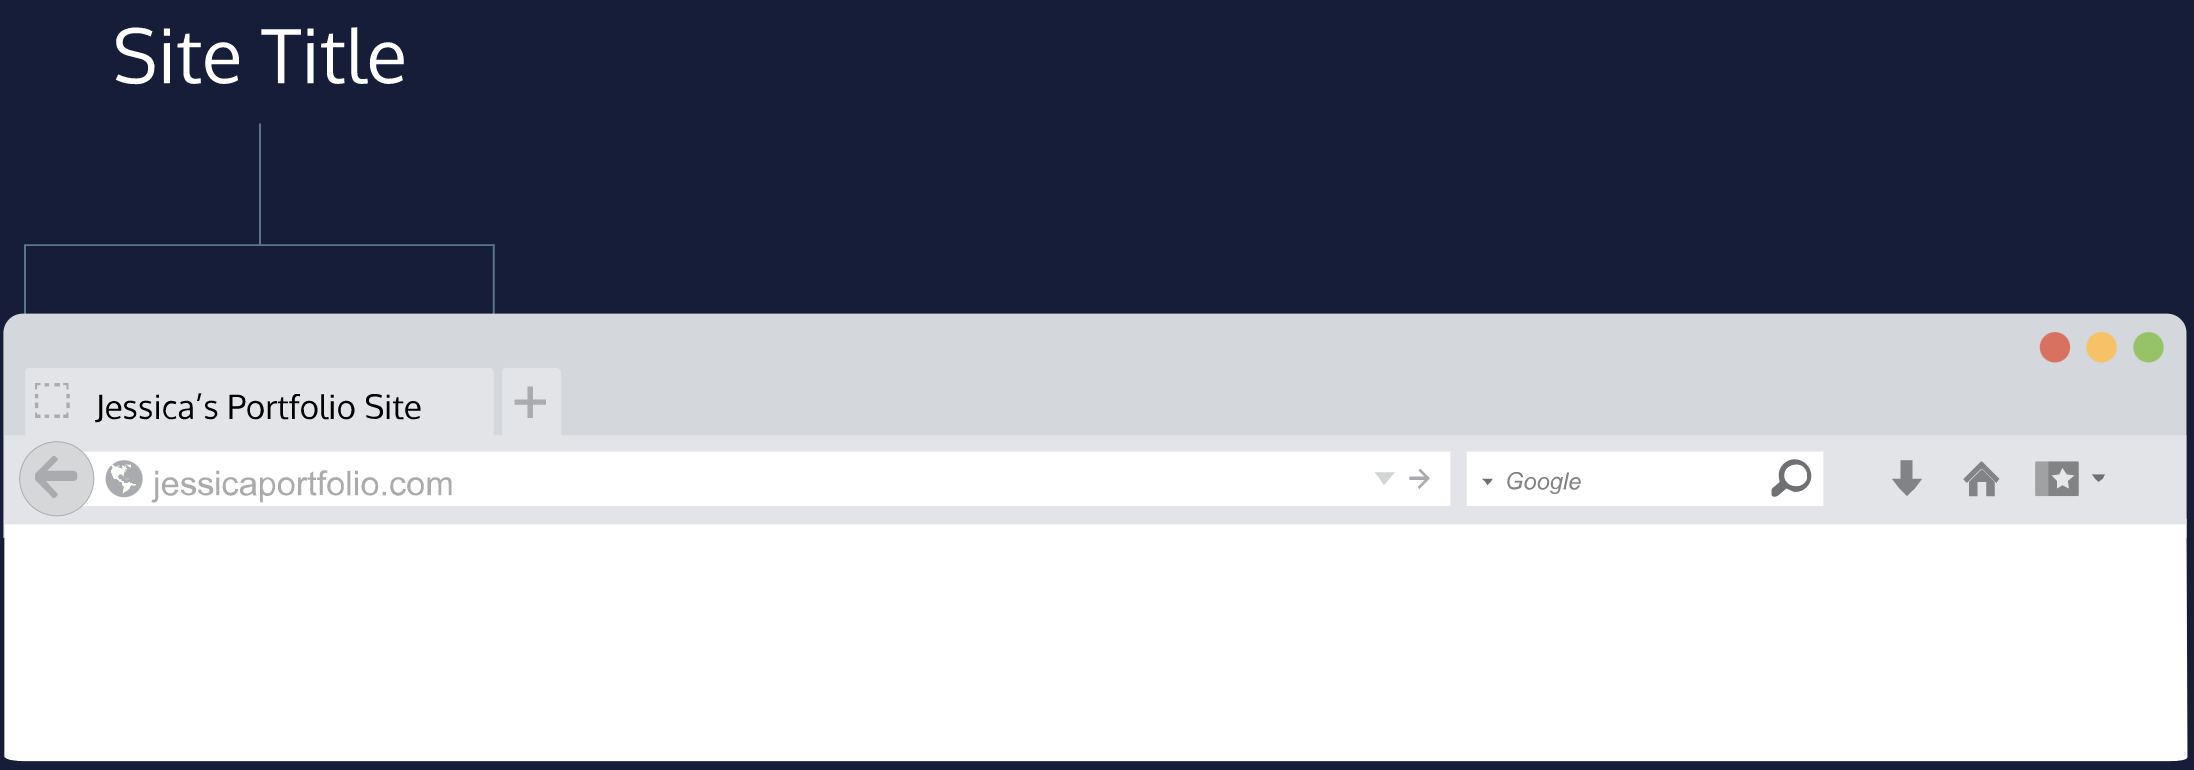
\includegraphics[scale = 0.4]{1_2}
\centering
\end{figure}
So far, we have learned about:
\begin{itemize}[leftmargin = *]
\item \colorbox{lightgray}{<!DOCTYPE html>}, the declaration specifying the version of HTML for the browser
\item The \colorbox{lightgray}{<html>} tags that enclose all of your HTML code
\item The \colorbox{lightgray}{<head>} tag that contains the metadata of a webpage, such as its \colorbox{lightgray}{<title>}
\end{itemize}
Next, we will learn about new types of elements that go inside the body.

\subsection{Linking to Other Web Pages}
One of the powerful aspects of HTML (and the Internet), is the ability to \textit{link} to other web pages.

We can add links to a web page by adding an \textit{anchor} element \colorbox{lightgray}{<a>} and including the text of the link in between the opening and closing tags.
\begin{lstlisting}
<a>This Is a Link To Wikipedia</a>
\end{lstlisting}
Technically, the link in the example above is incomplete. The link above cannot work because there is no URL that will lead users to the actual Wikipedia page. 

The anchor element in the example above is incomplete without the \colorbox{lightgray}{href} attribute. This attribute stands for \textit{hyperlink reference} and is used to link to a \textit{path}, or the address to where a file is located (whether it is on your computer or another location). The paths provided to the \colorbox{lightgray}{href} attribute are often URLs.
\begin{lstlisting}
<a href="https://www.wikipedia.org/">This Is a Link To Wikipedia</a>
\end{lstlisting}
In the example above, the \colorbox{lightgray}{href} attribute has been set to the value of the URL \colorbox{lightgray}{https://www.wikipedia.org/}. The example now shows the correct use of an anchor element.

When reading technical documentation, we may come across the term \textit{hyperlink}. This is simply the technical term for link, and these terms are often used interchangeably.

\subsection{Opening Links in a New Window}
Have you ever clicked on a link and observed the resulting web page open in a new browser window? If so, you can thank the \colorbox{lightgray}{<a>} element’s \colorbox{lightgray}{target} attribute.

The \colorbox{lightgray}{target} attribute specifies how a link should open.

It is possible that one or more links on your web page link to an entirely different website. In that case, you may want users to read the linked website, but hope that they return to your web page. This is exactly when the \colorbox{lightgray}{target} attribute is useful.

For a link to open in a new window, the \colorbox{lightgray}{target} attribute requires a value of \colorbox{lightgray}{\_blank}. The \colorbox{lightgray}{target} attribute can be added directly to the opening tag of the anchor element, just like the \colorbox{lightgray}{href} attribute.
\begin{lstlisting}
<a href="https://en.wikipedia.org/wiki/Brown_bear" 
target="_blank">The Brown Bear</a>
\end{lstlisting}
In the example above, setting the \colorbox{lightgray}{target} attribute to "\colorbox{lightgray}{\_blank}" instructs the browser to open the relevant Wikipedia page in a new window.

In this exercise, we have used the terminology “open in a new window.” It is likely that you are using a modern browser that opens up websites in new \textit{tabs}, rather than new windows. Before the advent of browsers with tabs, additional browser windows had to be opened to view more websites. The \colorbox{lightgray}{target="\_blank"} attribute, when used in modern browsers, will open new websites in a new tab.

\subsection{Linking to Relative Page}
Thus far we have learned how to link to external web pages. Many sites also link to internal web pages like Home, About, and Contact.

Before we learn how to link between internal pages, let us establish where our files are stored. When making multi-page static websites, web developers often store HTML files in the root directory, or a main folder where all the files for the project are stored. As the size of the projects you create grows, you may use additional folders within the main project folder to organize your code.
\begin{lstlisting}[basicstyle=\small\ttfamily\color{theWhite}, backgroundcolor = \color{theBlack}, language = Comment]
project-folder/
|__ about.html
|__ contact.html
|__ index.html
\end{lstlisting}
The example above shows three different files — \textbf{about.html}, \textbf{contact.html}, and \textbf{index.html} in one folder.

HTML files are often stored in the same folder, as shown in the example above. If the browser is currently displaying \textbf{index.html}, it also knows that \textbf{about.html} and \textbf{contact.html} are in the same folder. Because the files are stored in the same folder, we can link web pages together using a \textit{relative path}.
\begin{lstlisting}
<a href="./contact.html">Contact</a>
\end{lstlisting}
In this example, the \colorbox{lightgray}{<a>} tag is used with a relative path to link from the current HTML file to the \colorbox{lightgray}{contact.html} file in the same folder. On the web page, \colorbox{lightgray}{Contact} will appear as a link.

A relative path is a filename that shows the path to a \textit{local file} (a file on the same website, such as \colorbox{lightgray}{./index.htm}l) versus an absolute path (a full URL, like \colorbox{lightgray}{https://www.codecademy.com/learn/learn-html} which is stored in a different folder). The \colorbox{lightgray}{./} in \colorbox{lightgray}{./index.html} tells the browser to look for the file in the current folder.

\subsection{Linking At Will}
You have probably visited websites where not all links were made up of text. Maybe the links you clicked on were images or some other form of content.

So far, we have added links that were made up of only text, like the following:
\begin{lstlisting}
<a href="https://en.wikipedia.org/wiki/Opuntia"
target="_blank">Prickly Pear</a>
\end{lstlisting}
Text-only links, however, would significantly decrease our flexibility as web developers.

Thankfully, HTML allows us to turn nearly any element into a link by wrapping that element with an anchor element. With this technique, it is possible to turn images into links by simply wrapping the \colorbox{lightgray}{<img>} element with an \colorbox{lightgray}{<a>} element.
\begin{lstlisting}
<a href="https://en.wikipedia.org/wiki/Opuntia" 
target="_blank">(*@@*)<img
src="https://www.Prickly_Pear_Closeup.jpg" alt="A(*@ @*)red 
prickly(*@ @*)pear fruit"/></a>
\end{lstlisting}
In the example above, an image of a prickly pear has been turned into a link by wrapping the outside of the \colorbox{lightgray}{<img>} element with an \colorbox{lightgray}{<a>} element.

\subsection{Linking to Same Page}
At this point, we have all the content we want on our page. Since we have so much content, it does not all fit on the screen. How do we make it easier for a user to jump to different portions of our page?

When users visit our site, we want them to be able to click a link and have the page automatically scroll to a specific section.

In order to link to a target on the same page, we must give the target an \textit{id}, like this:
\begin{lstlisting}
<p id="top">This is the top of the page!</p>
<h1 id="bottom">This is the bottom! </h1>
\end{lstlisting}
In this example, the \colorbox{lightgray}{<p>} element is assigned an \colorbox{lightgray}{id} of “top” and the \colorbox{lightgray}{<h1>} element is assigned “bottom.” An \colorbox{lightgray}{id} can be added to most elements on a webpage.

An \colorbox{lightgray}{id} should be descriptive to make it easier to remember the purpose of a link. The target link is a string containing the \colorbox{lightgray}{\#} character and the target element’s \colorbox{lightgray}{id}.
\begin{lstlisting}
<ol>
  <li><a href="#top">Top</a></li>
  <li><a href="#bottom">Bottom</a></li>
</ol>
\end{lstlisting}
In the example above, the links to \colorbox{lightgray}{<p id="top">} and \colorbox{lightgray}{<h1 id="bottom">} are embedded in an ordered list. These links appear in the browser as a numbered list of links. An \colorbox{lightgray}{id} is especially helpful for organizing content belonging to a \colorbox{lightgray}{div}.

\subsection{Whitespace}
Now we will focus on some tools developers use to make code easier to interpret.

As the code in an HTML file grows, it becomes increasingly difficult to keep track of how elements are related. Programmers use two tools to visualize the relationship between elements: \textit{whitespace} and \textit{indentation}.

Both tools take advantage of the fact that the position of elements in a browser is independent of the amount of whitespace or indentation in an HTML file.

For example, if we wanted to increase the space between two paragraphs on your web page, you would not be able to accomplish this by adding space between the paragraph elements in the HTML file. The browser ignores whitespace in HTML files when it renders a web page, so it can be used as a tool to make code easier to read and follow.

What makes the example below difficult to read?
\begin{lstlisting}
<body><p>Paragraph 1</p><p>Paragraph 2</p></body>
\end{lstlisting}
We have to read the entire line to know what elements are present. Compare the example above to this:
\begin{lstlisting}
<body>
    <p>Paragraph 1</p>
    <p>Paragraph 2</p>
</body>
\end{lstlisting}
This example is easier to read, because each element is on its own line. While the first example required you to read the entire line of code to identify the elements, this example makes it easy to identify the body tag and two paragraphs.

A browser renders both examples the same way:
\begin{lstlisting}[basicstyle=\small\ttfamily\color{theWhite}, backgroundcolor = \color{theBlack}, language = Comment]
Paragraph 1
Paragraph 2
\end{lstlisting}
Next we will learn how to use indentation to help visualize nested elements.

\subsection{Indentation}
The second tool web developers use to make the structure of code easier to read is indentation. The spaces are inserted using the space and tab bars on your keyboard.

The \href{https://www.w3.org/Consortium/}{World Wide Web Consortium}, or W3C, is responsible for maintaining the style standards of HTML. At the time of writing, the W3C recommends 2 spaces of indentation when writing HTML code. Although your code will work without exactly two spaces, this standard is followed by the majority of professional web developers. Indentation is used to easily visualize which elements are nested within other elements.
\begin{lstlisting}
<body>
  <p>Paragraph 1</p>
  <div>
    <p>Paragraph 2</p>
  </div>
</body>
\end{lstlisting}
In the example above, \colorbox{lightgray}{Paragraph 1} and the \colorbox{lightgray}{<div>} tag are nested inside of the \colorbox{lightgray}{<body>} tag, so they are indented two spaces. The \colorbox{lightgray}{Paragraph 2} element is nested inside of the \colorbox{lightgray}{<div>} tag, so it is indented an additional two spaces.

\subsection{Comments}
HTML files also allow you to add comments to your code.

Comments begin with \colorbox{lightgray}{<!--} and end with \colorbox{lightgray}{-->}. Any characters in between will be ignored by your browser.
\begin{lstlisting}
<!-- This is a comment that the browser will not display. -->
\end{lstlisting}
Including comments in our code is helpful for many reasons:
\begin{enumerate}[leftmargin = *]
\item They help us (and others) understand our code if we decide to come back and review it at a much later date.
\item They allow us to experiment with new code, without having to delete old code.
\end{enumerate}
\begin{lstlisting}
<!-- Favorite Films Section -->
<p>The following is a list of my favorite films:</p>
\end{lstlisting}
In this example, the comment is used to denote that the following text makes up a particular section of the page.
\begin{lstlisting}
<!-- <p> Test Code </p> -->
\end{lstlisting}
In the example above, a valid HTML element (a paragraph element) has been “commented out.” This practice is useful when there is code you want to experiment with, or return to, in the future.

\subsection{HTML Tags}
We now know all of the basic elements and set-up we need to structure an HTML page and add different types of content. With the help of CSS, very soon we will be creating beautiful websites. 

While some tags have a very specific purpose, such as image and video tags, most tags are used to describe the content that they surround, which helps us modify and style our content later. There are seemingly infinite numbers of tags to use. Knowing when to use each one is based on how you want to describe the content of your HTML. Descriptive, well-chosen tags are one key to high-quality web development. A full list of available HTML tags can be found in \href{https://developer.mozilla.org/en-US/docs/Web/HTML/Element}{Mozilla documentation}.

Let us review what we have learned:
\begin{itemize}[leftmargin = *]
\item The \colorbox{lightgray}{<!DOCTYPE html>} declaration should always be the first line of code in our HTML files. This lets the browser know what version of HTML to expect.
\item The \colorbox{lightgray}{<html>} element will contain all of your HTML code.
\item Information about the web page, like the title, belongs within the \colorbox{lightgray}{<head>} of the page.
\item You can add a title to your web page by using the \colorbox{lightgray}{<title>} element, inside of the head.
\item A webpage’s title appears in a browser’s tab.
\item Anchor tags (\colorbox{lightgray}{<a>}) are used to link to internal pages, external pages or content on the same page.
\item You can create sections on a webpage and jump to them using \colorbox{lightgray}{<a>} tags and adding \colorbox{lightgray}{id}s to the elements you wish to jump to.
\item Whitespace between HTML elements helps make code easier to read while not changing how elements appear in the browser.
\item Indentation also helps make code easier to read. It makes parent-child relationships visible.
\item Comments are written in HTML using the following syntax: \colorbox{lightgray}{<!-- comment -->}.
\end{itemize}

\newpage
\section{HTML Tables}
Now we will learn how to use tables to present tabular data to users.
\subsection{Introduction to Tables}
There are many websites on the Internet that display information like stock prices, sports scores, invoice data, and more. This data is naturally tabular in nature, meaning that a table is often the best way of presenting the data. Now we will learn how to use the HTML \colorbox{lightgray}{<table>} element to present information in a two-dimensional table to the users.

\subsection{Create a Table}
Before displaying data, we must first create the table that will contain the data by using the \colorbox{lightgray}{<table>} element.
\begin{lstlisting}
<table>

</table>
\end{lstlisting}
The \colorbox{lightgray}{<table>} element will contain all of the tabular data we plan on displaying.

\subsection{Table Rows}
In many programs that use tables, the table is already predefined for you, meaning that it contains the \href{https://en.wikipedia.org/wiki/Table_(information)}{rows, columns, and cells that will hold data}. In HTML, all of these components must be created.

The first step in entering data into the table is to add rows using the table row element: \colorbox{lightgray}{<tr>}.
\begin{lstlisting}
<table>
  <tr>
  </tr>
  <tr>
  </tr>
</table>
\end{lstlisting}
In the example above, two rows have been added to the table.

\subsection{Table Data}
Rows are not sufficient to add data to a table. Each cell element must also be defined. In HTML, you can add data using the \textit{table data} element: \colorbox{lightgray}{<td>}.
\begin{lstlisting}
<table>
  <tr>
    <td>73</td>
    <td>81</td>
  </tr>
</table>
\end{lstlisting}
In the example above, two data points (\colorbox{lightgray}{73} and \colorbox{lightgray}{81}) were entered in the one row that exists. By adding two data points, we created two cells of data.

If the table were displayed in the browser, it would show a table with one row and two columns.

\subsection{Table Headings}
Table data does not make much sense without titles to describe what the data represents.

To add titles to rows and columns, you can use the table heading element: \colorbox{lightgray}{<th>}.

The table heading element is used just like a table data element, except with a relevant title. Just like table data, a table heading must be placed within a table row.
\begin{lstlisting}
<table>
  <tr>
    <th></th>
    <th scope="col">Saturday</th>
    <th scope="col">Sunday</th>
  </tr>
  <tr>
    <th scope="row">Temperature</th>
    <td>73</td>
    <td>81</td>
  </tr>
</table>
\end{lstlisting}

First, a new row was added to hold the three headings: a blank heading, a \colorbox{lightgray}{Saturday} heading, and a \colorbox{lightgray}{Sunday} heading. The blank heading creates the extra table cell necessary to align the table headings correctly over the data they correspond to.

In the second row, one table heading was added as a row title: \colorbox{lightgray}{Temperature}.

Note, also, the use of the scope attribute, which can take one of two values:
\begin{enumerate}[leftmargin = *]
\item \colorbox{lightgray}{row} - this value makes it clear that the heading is for a row.
\item \colorbox{lightgray}{col} - this value makes it clear that the heading is for a column.
\end{enumerate}
HTML code for tables may look a little strange at first, but analyzing it piece by piece helps make the code more understandable.

\subsection{Table Borders}
So far, the tables we have created have been a little difficult to read because they have no borders.

In older versions of HTML, a border could be added to a table using the \colorbox{lightgray}{border} attribute and setting it equal to an integer. This integer would represent the thickness of the border.
\begin{lstlisting}
<table border="1">
  <tr>
    <td>73</td>
    <td>81</td>
  </tr>
</table>
\end{lstlisting}
The code in the example above is \href{https://en.wikipedia.org/wiki/Deprecation}{deprecated}, so please do not use it. It is meant to illustrate older conventions you may come across when reading other developers’ code.

The browser will likely still interpret your code correctly if you use the \colorbox{lightgray}{border} attribute, but that does not mean the attribute should be used.

We use CSS to add style to HTML documents, because it helps us to separate the structure of a page from how it looks. You can achieve the same table border effect using CSS.
\begin{lstlisting}
table, td {
  border: 1px solid black;
}
\end{lstlisting}
The code in the example above uses CSS instead of HTML to show table borders.

\subsection{Spanning Columns}
Next let us investigate the case where the table contains data that spans multiple columns. 

For example, a personal calendar could have events that span across multiple hours, or even multiple days.

Data can span columns using the \colorbox{lightgray}{colspan} attribute. The attributes accepts an integer (greater than or equal to 1) to denote the number of columns it spans across.
\begin{lstlisting}
<table>
  <tr>
    <th>Monday</th>
    <th>Tuesday</th>
    <th>Wednesday</th>
  </tr>
  <tr>
    <td colspan="2">Out of Town</td>
    <td>Back in Town</td>
  </tr>
</table>
\end{lstlisting}
In the example above, the data \colorbox{lightgray}{Out of Town} spans the \colorbox{lightgray}{Monday} and \colorbox{lightgray}{Tuesday} table headings using the value \colorbox{lightgray}{2} (two columns). The data \colorbox{lightgray}{Back in Town} appear only under the \colorbox{lightgray}{Wednesday} heading.

\subsection{Spanning Rows}
Data can also span multiple rows using the \colorbox{lightgray}{rowspan} attribute.

The \colorbox{lightgray}{rowspan} attribute is used for data that spans multiple rows (perhaps an event goes on for multiple hours on a certain day). It accepts an integer (greater than or equal to 1) to denote the number of rows it spans across.
\begin{lstlisting}
<table>
  <tr> <!-- Row 1 -->
    <th></th>
    <th>Saturday</th>
    <th>Sunday</th>
  </tr>
  <tr> <!-- Row 2 -->
    <th>Morning</th>
    <td rowspan="2">Work</td>
    <td rowspan="3">Relax</td>
  </tr>
  <tr> <!-- Row 3 -->
    <th>Afternoon</th>
  </tr>
  <tr> <!-- Row 4 -->
    <th>Evening</th>
    <td>Dinner</td>
  </tr>
</table>
\end{lstlisting}
In the example above, there are four rows:
\begin{enumerate}[leftmargin = *]
\item The first row contains an empty cell and the two column headings.
\item The second row contains the \colorbox{lightgray}{Morning} row heading, along with \colorbox{lightgray}{Work}, which spans two rows under the \colorbox{lightgray}{Saturday} column. The “Relax” entry spans three rows under the \colorbox{lightgray}{Sunday} column.
\item The third row only contains the \colorbox{lightgray}{Afternoon} row heading.
\item The fourth row only contains the \colorbox{lightgray}{Dinner} entry, since “Relax” spans into the cell next to it.
\end{enumerate}
\begin{figure}[H]
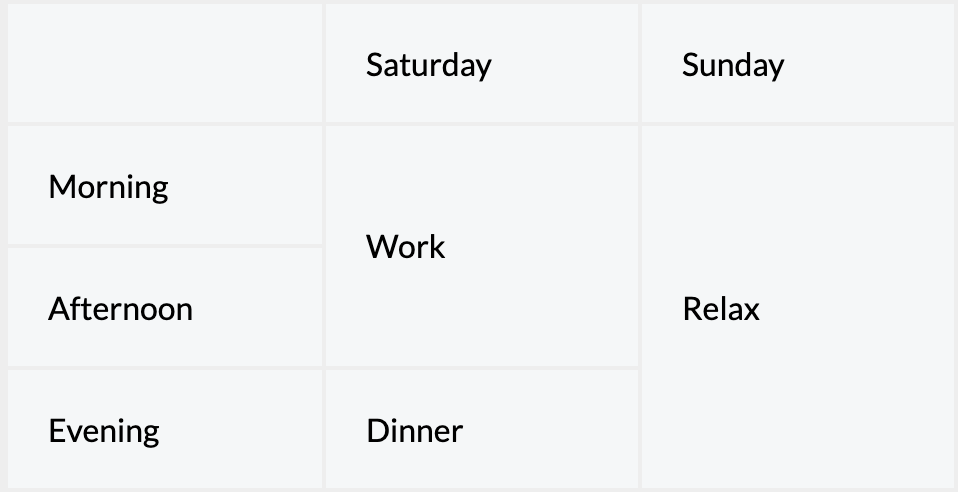
\includegraphics[scale = 0.7]{3_1}
\centering
\end{figure}

\subsection{Table Body}
Over time, a table can grow to contain a lot of data and become very long. When this happens, the table can be sectioned off so that it is easier to manage.

Long tables can be sectioned off using the \textit{table body} element: \colorbox{lightgray}{<tbody>}.

The \colorbox{lightgray}{<tbody>} element should contain all of the table’s data, excluding the table headings.
\begin{lstlisting}
<table>
  <tbody>
    <tr>
      <th></th>
      <th>Saturday</th>
      <th>Sunday</th>
    </tr>
    <tr>
      <th>Morning</th>
      <td rowspan="2">Work</td>
      <td rowspan="3">Relax</td>
    </tr>
    <tr>
     <th>Afternoon</th>
    </tr>
    <tr>
      <th>Evening</th>
      <td>Dinner</td>
    </tr>
  </tbody>
</table>
\end{lstlisting}
In the example above, all of the table data is contained within a table body element. Note, however, that the headings were also kept in the table’s body.

\subsection{Table Head}
Previously, the table’s headings were kept inside of the table’s body. When a table’s body is sectioned off, however, it also makes sense to section off the table’s column headings using the \colorbox{lightgray}{<thead>} element.
\begin{lstlisting}
<table>
  <thead>
    <tr>
      <th></th>
      <th scope="col">Saturday</th>
      <th scope="col">Sunday</th>
    </tr>
  </thead>
  <tbody>
    <tr>
      <th scope="row">Morning</th>
      <td rowspan="2">Work</td>
      <td rowspan="3">Relax</td>
    </tr>
    <tr>
     <th scope="row">Afternoon</th>
    </tr>
    <tr>
      <th scope="row">Evening</th>
      <td>Dinner</td>
    </tr>
  </tbody>
</table>
\end{lstlisting}
In the example above, the only new element is \colorbox{lightgray}{<thead>}. The table headings are contained inside of this element. Note that the table’s head still requires a row in order to contain the table headings.

Additionally, only the \textbf{column} headings go under the \colorbox{lightgray}{<thead>} element. We can use the \colorbox{lightgray}{scope} attribute on \colorbox{lightgray}{<th>} elements to indicate whether a \colorbox{lightgray}{<th>} element is being used as a \colorbox{lightgray}{"row"} heading or a \colorbox{lightgray}{"col"} heading.

\subsection{Table Footer}
The bottom part of a long table can also be sectioned off using the \colorbox{lightgray}{<tfoot>} element.
\begin{lstlisting}
<table>
  <thead>
    <tr>
      <th>Quarter</th>
      <th>Revenue</th>
      <th>Costs</th>
    </tr>
  </thead>
  <tbody>
    <tr>
      <th>Q1</th>
      <td>$10M</td>
      <td>$7.5M</td>
    </tr>
    <tr>
      <th>Q2</th>
      <td>$12M</td>
      <td>$5M</td>
    </tr>
  </tbody>
  <tfoot>
    <tr>
      <th>Total</th>
      <td>$22M</td>
      <td>$12.5M</td>
    </tr>
  </tfoot>
</table>
\end{lstlisting}
In the example above, the footer contains the totals of the data in the table. Footers are often used to contain sums, differences, and other data results.

\subsection{Styling with CSS}
Tables, by default, are very bland. They have no borders, the font color is black, and the typeface is the same type used for other HTML elements.

We can use CSS to style tables. Specifically, we can style the various aspects mentioned above.
\begin{lstlisting}
table, th, td {
  border: 1px solid black;
  font-family: Arial, sans-serif;
  text-align: center;
}
\end{lstlisting}
The code in the example above demonstrates just some of the various table aspects we can style using CSS properties.

\subsection{Review}
We learned how to create a table, add data to it, and section the table into smaller parts that make it easier to read.

Let is review what this chapter covered:
\begin{itemize}[leftmargin = *]
\item The \colorbox{lightgray}{<table>} element creates a table.
\item The \colorbox{lightgray}{<tr>} element adds rows to a table.
\item To add data to a row, you can use the \colorbox{lightgray}{<td>} element.
\item Table headings clarify the meaning of data. Headings are added with the \colorbox{lightgray}{<th>} element.
\item Table data can span columns using the \colorbox{lightgray}{colspan} attribute.
\item Table data can span rows using the \colorbox{lightgray}{rowspan} attribute.
\item Tables can be split into three main sections: a head, a body, and a footer.
\item A table’s head is created with the \colorbox{lightgray}{<thead>} element.
\item A table’s body is created with the \colorbox{lightgray}{<tbody>} element.
\item A table’s footer is created with the \colorbox{lightgray}{<tfoot>} element.
\item All the CSS properties you learned about in this course can be applied to tables and their data.
\end{itemize}

\newpage
\section{HTML Forms}
Now we will cover how to add a \colorbox{lightgray}{<form>} element populated with various elements that accept input on a web page.
\subsection{Introduction to HTML Forms}
Forms are a part of everyday life. When we use a physical form in real life, we write down information and give it to someone to process. Think of the times you have had to fill out information for various applications like a job, or a bank account, or dropped off a completed suggestion card — each instance is a form.

Just like a physical form, an HTML \colorbox{lightgray}{<form>} element is responsible for collecting information to send somewhere else. Every time we browse the internet we come into contact with many forms and we might not even realize it. There is a good chance that if we are typing into a text field or providing an input, the field that we are typing into is part of a \colorbox{lightgray}{<form>}.

Now we will go over the structure and syntax of a \colorbox{lightgray}{<form>} and the many elements that populate it.

\subsection{How a Form Works}
We can think of the internet as a network of computers which send and receive information. Computers need an \textit{HTTP request} to know how to communicate. The HTTP request instructs the receiving computer how to handle the incoming information. More information can be found in the article about \href{https://www.codecademy.com/articles/http-requests}{HTTP requests}.

The \colorbox{lightgray}{<form>} element is a great tool for collecting information, but then we need to send that information somewhere else for processing. We need to supply the \colorbox{lightgray}{<form>} element with both the location of where the \colorbox{lightgray}{<form>}'s information goes and what HTTP request to make. Take a look at the sample \colorbox{lightgray}{<form>} below:
\begin{lstlisting}
<form action="/example.html" method="POST">
</form>
\end{lstlisting}
In the above example, we have created the skeleton for a \colorbox{lightgray}{<form>} that will send information to \textbf{example.html} as a POST request:
\begin{itemize}[leftmargin = *]
\item The \colorbox{lightgray}{action} attribute determines where the information is sent.
\item The \colorbox{lightgray}{method} attribute is assigned a HTTP verb that is included in the HTTP request.
\end{itemize}
Note: HTTP verbs like POST do not need to be capitalized for the request to work, but it is done so out of convention. In the example above we could have written \colorbox{lightgray}{method="post"} and it would still work.

The \colorbox{lightgray}{<form>} element can also contain child elements. For instance, it would be helpful to provide a header so that users know what this \colorbox{lightgray}{<form>} is about. We could also add a paragraph to provide even more detail. Let us see an example of this in code:
\begin{lstlisting}
<form action="/example.html" method="POST">
  <h1>Creating a form</h1>
  <p>Looks like you want to learn how to create an HTML form. Well, the best way to learn is to play around with it.</p>
</form>
\end{lstlisting}

\subsection{Text Input}
If we want to create an input field in our \colorbox{lightgray}{<form>}, we will need the help of the \colorbox{lightgray}{<input>} element.

The \colorbox{lightgray}{<input>} element has a \colorbox{lightgray}{type} attribute which determines how it renders on the web page and what kind of data it can accept.

The first value for the \colorbox{lightgray}{type} attribute we are going to explore is \colorbox{lightgray}{"text"}. When we create an \colorbox{lightgray}{<input>} element with \colorbox{lightgray}{type="text"}, it renders a text field that users can type into. It is also important that we include a name attribute for the \colorbox{lightgray}{<input>} — without the name attribute, information in the \colorbox{lightgray}{<input>} will not be sent when the \colorbox{lightgray}{<form>} is submitted. We will explain more about submissions and the submit button later. For now, let us examine the following code that produces a text input field:
\begin{lstlisting}
<form action="/example.html" method="POST">
  <input type="text" name="first-text-field">
</form>
\end{lstlisting}
Here is a screen shot of how the rendered form looks like on a web page for the Chrome browser (different browsers have different default rendering). When initially loaded, it will be an empty box:
\begin{figure}[H]
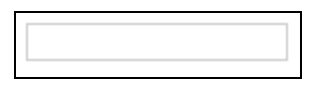
\includegraphics[scale = 0.5]{3_2}
\centering
\end{figure}
\vspace{-4mm}
After users type into the \colorbox{lightgray}{<input>} element, the value of the \colorbox{lightgray}{value} attribute becomes what is typed into the text field. The value of the \colorbox{lightgray}{value} attribute is paired with the value of the \colorbox{lightgray}{name} attribute and sent as text when the form is submitted. For instance, if a user typed in “important details” in the text field created by our \colorbox{lightgray}{<input>} element:
\begin{figure}[H]
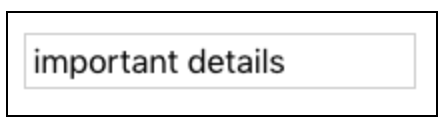
\includegraphics[scale = 0.5]{3_3}
\centering
\end{figure}
\vspace{-4mm}
When the form is submitted, the text: \colorbox{lightgray}{"first-text-field=important details"} is sent to \colorbox{lightgray}{/example.html} because the value of the name attribute is \colorbox{lightgray}{"first-text-field"} and the value of value is \colorbox{lightgray}{"important details"}.

We could also assign a default value for the \colorbox{lightgray}{value} attribute so that users have a pre-filled text field when they first see the rendered form like so:
\begin{lstlisting}
<form action="/example.html" method="POST">
  <input type="text" name="first-text-field" value="already pre-filled">
</form>
\end{lstlisting}
This renders:
\begin{figure}[H]
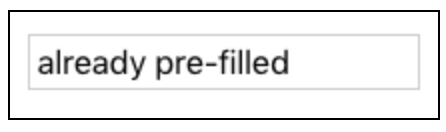
\includegraphics[scale = 0.5]{3_4}
\centering
\end{figure}
\vspace{-4mm}

\subsection{Adding a Label}
Previously we created an \colorbox{lightgray}{<input>} element but we did not include anything to explain what the \colorbox{lightgray}{<input>} is used for. For a user to properly identify an \colorbox{lightgray}{<input>} we use the appropriately named \colorbox{lightgray}{<label>} element.

The \colorbox{lightgray}{<label>} element has an opening and closing tag and displays text that is written between the opening and closing tags. To associate a \colorbox{lightgray}{<label>} and an \colorbox{lightgray}{<input>}, the \colorbox{lightgray}{<input>} needs an \colorbox{lightgray}{id} attribute. We then assign the \colorbox{lightgray}{for} attribute of the \colorbox{lightgray}{<label>} element with the value of the \colorbox{lightgray}{id} attribute of \colorbox{lightgray}{<input>}, like so:
\begin{lstlisting}
<form action="/example.html" method="POST">
  <label for="meal">What do you want to eat?</label>
  <br>
  <input type="text" name="food" id="meal">
</form>
\end{lstlisting}
The code above renders:
\begin{figure}[H]
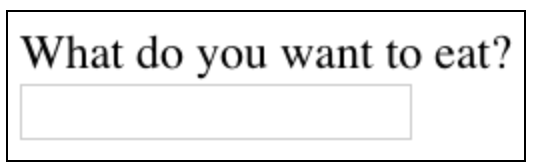
\includegraphics[scale = 0.5]{3_5}
\centering
\end{figure}
\vspace{-4mm}
Now users know what the \colorbox{lightgray}{<input>} element is for. Another benefit for using the \colorbox{lightgray}{<label>} element is when this element is clicked, the corresponding \colorbox{lightgray}{<input>} is highlighted/selected.

\subsection{Password Input}
Think about all those times we have to put sensitive information, like a password or PIN, into a \colorbox{lightgray}{<form>}. We would not want our information to be seen by anyone peeking over our shoulder. Luckily, we have the \colorbox{lightgray}{type="password"} attribute for \colorbox{lightgray}{<input>}.

An \colorbox{lightgray}{<input type ="password">} element will replace input text with another character like an asterisk (*) or a dot (•). The code below provides an example of how to create a password field:
\begin{lstlisting}
<form>
  <label for="user-password">Password: </label>
  <input type="password" id="user-password" name="user-password">
</form>
\end{lstlisting}
After a user types into the field, it would look like:
\begin{figure}[H]
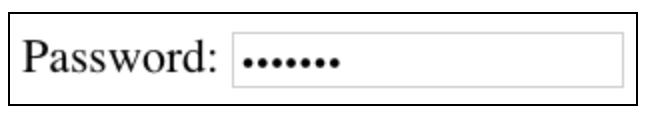
\includegraphics[scale = 0.5]{3_6}
\centering
\end{figure}
\vspace{-4mm}
Even though the password field obscures the text of the password, when the form is submitted, the value of the text is sent. In other words, if “hunter2” is typed into the password field, “user-password=hunter2” is sent along with the other information on the form.

\subsection{Number Input}
We have now gone over two type attributes for \colorbox{lightgray}{<input>} related to text. But, we might want our users to type in a number — in which case we can set the type attribute to \colorbox{lightgray}{"number"}. 

By setting \colorbox{lightgray}{type="number"} for an \colorbox{lightgray}{<input>} we can restrict what users type into the input field to just numbers (and a few special characters like \colorbox{lightgray}{$-$}, \colorbox{lightgray}{$+$}, and \colorbox{lightgray}{$.$}). We can also provide a \colorbox{lightgray}{step} attribute which creates arrows inside the input field to increase or decrease by the value of the \colorbox{lightgray}{step} attribute. Below is the code needed to render an input field for numbers:
\begin{lstlisting}
<form>
  <label for="years"> Years of experience: </label>
  <input id="years" name="years" type="number" step="1">
</form>
\end{lstlisting}
The code above renders:
\begin{figure}[H]
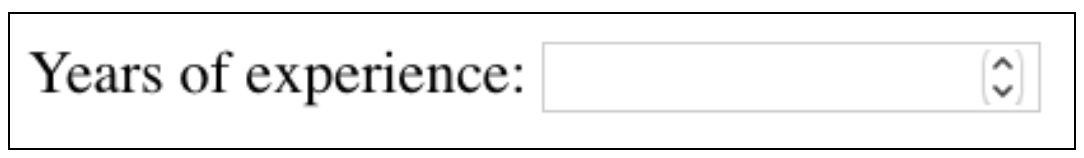
\includegraphics[scale = 0.4]{3_7}
\centering
\end{figure}
\vspace{-4mm}

\subsection{Range Input}
Using an \colorbox{lightgray}{<input type="number">} is great if we want to allow users to type in any number of their choosing. But, if we wanted to limit what numbers our users could type we might consider using a different type value. Another option we could use is setting \colorbox{lightgray}{type} to \colorbox{lightgray}{"range"} which creates a slider.

To set the minimum and maximum values of the slider we assign values to the \colorbox{lightgray}{min} and \colorbox{lightgray}{max} attribute of the \colorbox{lightgray}{<input>}. We could also control how smooth and fluid the slider works by assigning the \colorbox{lightgray}{step} attribute a value. Smaller \colorbox{lightgray}{step} values will make the slider more fluidly, whereas larger \colorbox{lightgray}{step} values will make the slider move more noticeably. Take a look at the code to create a slider:
\begin{lstlisting}
<form>
  <label for="volume"> Volume Control</label>
  <input id="volume" name="volume" type="range" min="0" max="100" step="1">
</form>
\end{lstlisting}
The code above renders: 
\begin{figure}[H]
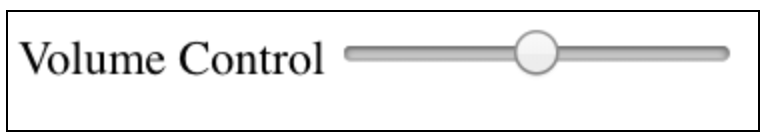
\includegraphics[scale = 0.5]{3_8}
\centering
\end{figure}
\vspace{-4mm}
In the example above, every time the slider moves by one, the value of the \colorbox{lightgray}{<input>}'s \colorbox{lightgray}{value} attribute changes.

\subsection{Checkbox Input}
So far the types of inputs we have allowed were all single choices. But, what if we presented multiple options to users and allow them to select any number of options? Sounds like we could use checkboxes. In a \colorbox{lightgray}{<form>} we would use the \colorbox{lightgray}{<input>} element and set \colorbox{lightgray}{type="checkbox"}. Examine the code used to create multiple checkboxes:
\begin{lstlisting}
<form>
  <p>Choose your pizza toppings:</p>
  <label for="cheese">Extra cheese</label>
  <input id="cheese" name="topping" type="checkbox" value="cheese">
  <br>
  <label for="pepperoni">Pepperoni</label>
  <input id="pepperoni" name="topping" type="checkbox" value="pepperoni">
  <br>
  <label for="anchovy">Anchovy</label>
  <input id="anchovy" name="topping" type="checkbox" value="anchovy">
</form>
\end{lstlisting}
The code above renders:
\begin{figure}[H]
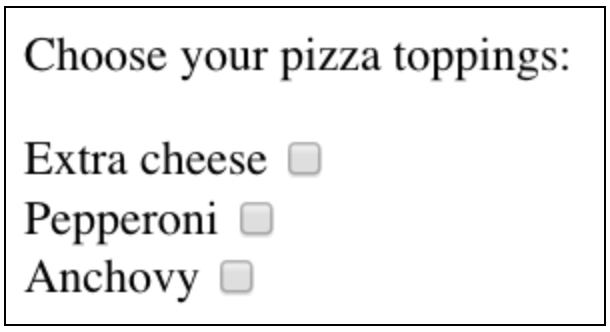
\includegraphics[scale = 0.5]{3_9}
\centering
\end{figure}
\vspace{-4mm}
Notice in the example provided:
\begin{itemize}[leftmargin = *]
\item there are assigned values to the \colorbox{lightgray}{value} attribute of the checkboxes. These values are not visible on the form itself, that is why it is important that we use an associated \colorbox{lightgray}{<label>} to identify the checkbox.
\item each \colorbox{lightgray}{<input>} has the same value for the \colorbox{lightgray}{name} attribute. Using the same \colorbox{lightgray}{name} for each checkbox groups the \colorbox{lightgray}{<input>}s together. However, each \colorbox{lightgray}{<input>} has a unique \colorbox{lightgray}{id} to pair with a \colorbox{lightgray}{<label>}.
\end{itemize}

\subsection{Radio Button Input}
Checkboxes work well if we want to present users with multiple options and let them choose one or more of the options. However, there are cases where we want to present multiple options and only allow for one selection — like asking users if they agree or disagree with the terms and conditions. Let us look over the code used to create radio buttons:
\begin{lstlisting}
<form>
  <p>What is sum of 1 + 1?</p>
  <input type="radio" id="two" name="answer" value="2">
  <label for="two">2</label>
  <br>
  <input type="radio" id="eleven" name="answer" value="11">
  <label for="eleven">11</label>
</form>
\end{lstlisting}
The code above renders:
\begin{figure}[H]
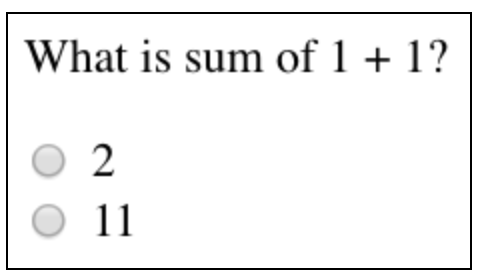
\includegraphics[scale = 0.5]{3_10}
\centering
\end{figure}
\vspace{-4mm}
Notice from the code snippet, radio buttons (like checkboxes) do not display their value. We have an associated \colorbox{lightgray}{<label>} to represent the value of the radio button. To group radio buttons together, we assign them the same \colorbox{lightgray}{name} and only one radio button from that group can be selected.

\subsection{Dropdown list}
Radio buttons are great if we want our users to pick one option out of a few visible options, but imagine if we have a whole list of options. This situation could quickly lead to a lot of radio buttons to keep track of. 

An alternative solution is to use a dropdown list to allow our users to choose one option from an organized list. Here is the code to create a dropdown menu:
\begin{lstlisting}
<form>
  <label for="lunch">What's for lunch?</label>
  <select id="lunch" name="lunch">
    <option value="pizza">Pizza</option>
    <option value="curry">Curry</option>
    <option value="salad">Salad</option>
    <option value="ramen">Ramen</option>
    <option value="tacos">Tacos</option>
  </select>
</form>
\end{lstlisting}
The code above renders:
\begin{figure}[H]
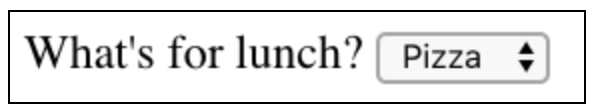
\includegraphics[scale = 0.5]{3_11}
\centering
\end{figure}
\vspace{-4mm}
And if we click on the field containing the first option, the list is revealed:
\begin{figure}[H]
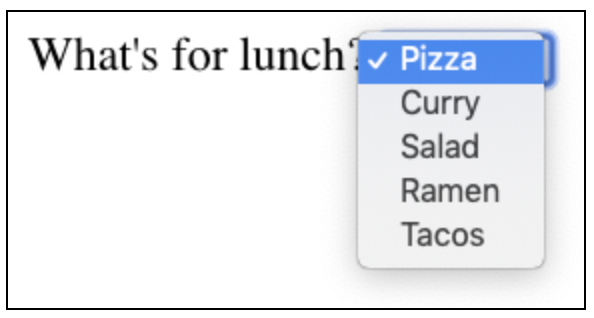
\includegraphics[scale = 0.5]{3_12}
\centering
\end{figure}
\vspace{-4mm}
Notice in the code that we are using the element \colorbox{lightgray}{<select>} to create the dropdown list. To populate the dropdown list, we add multiple \colorbox{lightgray}{<option>} elements, each with a \colorbox{lightgray}{value} attribute. By default, only one of these options can be selected.

The text rendered is the text included between the opening and closing \colorbox{lightgray}{<option>} tags. However, it is the \colorbox{lightgray}{value} of the \colorbox{lightgray}{value} attribute that is used in \colorbox{lightgray}{<form>} submission (notice the difference in the text and \colorbox{lightgray}{value} capitalization). When the \colorbox{lightgray}{<form>} is submitted, the information from this input field will be sent using the \colorbox{lightgray}{name} of the \colorbox{lightgray}{<select>} and the \colorbox{lightgray}{value} of the chosen \colorbox{lightgray}{<option>}. For instance, if a user selected Pizza from the dropdown list, the information would be sent as \colorbox{lightgray}{"lunch=pizza"}.

\subsection{Datalist Input}
Even if we have an organized dropdown list, if the list has a lot of options, it could be tedious for users to scroll through the entire list to locate one option. That is where using the \colorbox{lightgray}{<datalist>} element comes in handy.

The \colorbox{lightgray}{<datalist>} is used with an \colorbox{lightgray}{<input type="text">} element. The \colorbox{lightgray}{<input>} creates a text field that users can type into and filter options from the \colorbox{lightgray}{<datalist>}. Let us go over a concrete example:
\begin{lstlisting}
<form>
  <label for="city">Ideal city to visit?</label>
  <input type="text" list="cities" id="city" name="city">

  <datalist id="cities">
    <option value="New York City"></option>
    <option value="Tokyo"></option>
    <option value="Barcelona"></option>
    <option value="Mexico City"></option>
    <option value="Melbourne"></option>
    <option value="Other"></option>  
  </datalist>
</form>
\end{lstlisting}
Notice, in the code above, we have an \colorbox{lightgray}{<input>} that has a \colorbox{lightgray}{list} attribute. The \colorbox{lightgray}{<input>} is associated to the \colorbox{lightgray}{<datalist>} via the \colorbox{lightgray}{<input>}'s list attribute and the id of the \colorbox{lightgray}{<datalist>}.

From the code provided, the following form is rendered:
\begin{figure}[H]
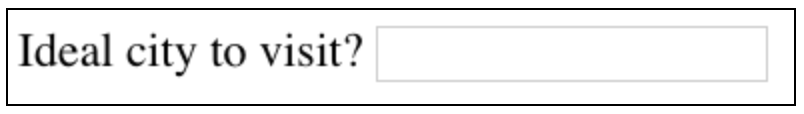
\includegraphics[scale = 0.5]{3_13}
\centering
\end{figure}
\vspace{-4mm}
And when field is selected:
\begin{figure}[H]
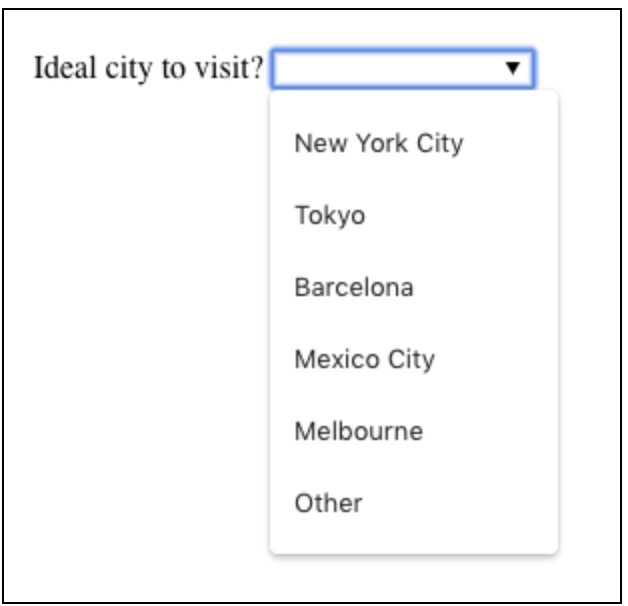
\includegraphics[scale = 0.5]{3_14}
\centering
\end{figure}
\vspace{-4mm}
While \colorbox{lightgray}{<select>} and \colorbox{lightgray}{<datalist>} share some similarities, there are some major differences. In the associated \colorbox{lightgray}{<input>} element, users can type in the input field to search for a particular option. If none of the \colorbox{lightgray}{<option>}s match, the user can still use what they typed in. When the form is submitted, the value of the \colorbox{lightgray}{<input>}'s \colorbox{lightgray}{name} and the \colorbox{lightgray}{value} of the option selected, or what the user typed in, is sent as a pair.

\subsection{Textarea element}
An \colorbox{lightgray}{<input>} element with \colorbox{lightgray}{type="text"} creates a single row input field for users to type in information. However, there are cases where users need to write in more information, like a blog post. In such cases, instead of using an \colorbox{lightgray}{<input>}, we could use \colorbox{lightgray}{<textarea>}.

The \colorbox{lightgray}{<textarea>} element is used to create a bigger text field for users to write more text. We can add the attributes rows and cols to determine the amount of rows and columns for the \colorbox{lightgray}{<textarea>}. Take a look:
\begin{lstlisting}
<form>
  <label for="blog">New Blog Post: </label>
  <br>
  <textarea id="blog" name="blog" rows="5" cols="30">
  </textarea>
</form>
\end{lstlisting}
In the code above, an empty \colorbox{lightgray}{<textarea>} that is 5 rows by 30 columns is rendered to the page like so:
\begin{figure}[H]
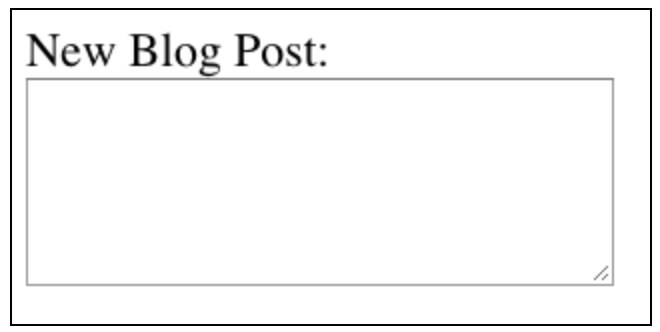
\includegraphics[scale = 0.5]{3_15}
\centering
\end{figure}
\vspace{-4mm}
If we wanted an even bigger text field, we could click and drag on the bottom right corner to expand it.

When we submit the form, the value of \colorbox{lightgray}{<textarea>} is the text written inside the box. If we want to add a default value to text to \colorbox{lightgray}{<textarea>} we would include it within the opening and closing tags like so:
\begin{lstlisting}
<textarea>Adding default text</textarea>
\end{lstlisting}
This code will render a \colorbox{lightgray}{<textarea>} that contains pre-filled text: “Adding default text”.



\end{document}
